\documentclass[serif,mathserif]{beamer}
\usepackage{amsmath, amsfonts, epsfig, xspace}
\usepackage{algorithm,algorithmic}
\usepackage{pstricks,pst-node}
\usepackage{multimedia}
\usepackage[normal,tight,center]{subfigure}
\setlength{\subfigcapskip}{-.5em}
\usepackage{beamerthemesplit}
\usetheme{lankton-keynote}
\usepackage{graphicx,color}
% remove caption of figure
\usepackage[labelformat=empty]{caption}

\usepackage[none]{hyphenat} % hyphenation is ugly in slides
\usepackage{parskip}

\usepackage{relsize} % \smaller to change size

\usepackage{tikz}
\usetikzlibrary{calc}

\usetikzlibrary{arrows}

\newcommand{\TikzDraw}[2][]{
  \begin{tikzpicture}[overlay, remember picture, shift={(current page.center)}, #1]
    #2
  \end{tikzpicture}
}

\newcommand{\gridlines}{
  \TikzDraw{
    \draw[help lines,xstep=.2,ystep=.2,red!20] (current page.south west) grid (current page.north east);
    \draw[help lines,xstep=1,ystep=1,red] (current page.south west) grid (current page.north east);
    \foreach \x in {-15,-14,...,15} {
      \node [anchor=north, red] at (\x,0) {\tiny \x};
      \node [anchor=east,red] at (0,\x) {\tiny \x};
    }
  }
}

\newcommand{\DrawOnImg}[3][]
{
  \begin{tikzpicture}
    \node[anchor=south west,inner sep=0] (image) at (0,0){
      #2
    };
    \begin{scope}[x={(image.south east)},y={(image.north west)}]
      \ifthenelse{\equal{#1}{grid}}
                 {\draw[color=blue, style=dashed] (0,0) grid[xstep=.1, ystep=.1] (1.0001,1.0001);}
                 {}
                 #3
    \end{scope}
  \end{tikzpicture}
}


\author[Jiong Chen]{Jiong Chen}

\title[\hspace{2em}\insertframenumber/\inserttotalframenumber]{Projective Dynamics: Fusing Constraint Projections for Fast Simulation}

\date{September 30, 2015} %leave out for today's date to be insterted

% \institute{Justice League of America}

\begin{document}

\maketitle

% \section{Introduction}  % add these to see outline in slides

\begin{frame}
  \frametitle{Position Based Dynamics}
  \begin{itemize}
    \item Force based.
      \begin{equation*}
	\text{force} \rightarrow \text{acceleration} \rightarrow \text{velocity} \rightarrow \text{position}
      \end{equation*}
    \item Position based: stable, robust, fast, visually plausible...
  \end{itemize}
  \begin{figure}[t]
      \centering
      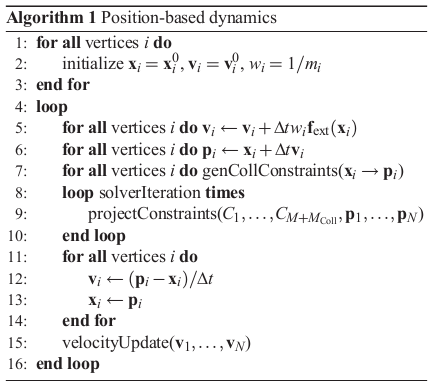
\includegraphics[scale=0.4]{pic/pbd.png}
  \end{figure}
\end{frame}

% \section{Main Body} % add these to see outline in slides

\begin{frame}
  \frametitle{Fast Simulation of Mass-Spring Systems}
  \begin{itemize}
   \item Reformulate spring potential with an auxiliary variable representing direction
    \begin{equation*}
     (\|\mathbf{p_1}-\mathbf{p_2}\|-r)^2=\underset{\|\mathbf{d}\|=r}\min~\|\mathbf{p_1}-\mathbf{p_2}-\mathbf{d}\|^2
    \end{equation*}
   with the analytic optimal solution
   \begin{equation*}
    \mathbf{d}^* = r(\mathbf{p_{12}}/\|\mathbf{p_{12}}\|)
   \end{equation*}
  The dynamics of the system then can be captured by alternating optimizing
  \begin{equation*}
   E(\mathbf{x}) = T(\mathbf{x},t)+\min_{\mathbf{d}}\frac{1}{2}\sum_{i=1}^s k_i\|\mathbf{p}_{i_1}-\mathbf{p}_{i_2}-\mathbf{d}_i\|^2+V_{other}(\mathbf{x})
  \end{equation*}

  \end{itemize}
\end{frame}

%\begin{frame}
%  \frametitle{Pictures}
%  \begin{figure}[t]
%    \centering
%    \subfigure[First Frame]{
%    \includegraphics[width=3cm]{figures/naked_leaves/00000001}}
%    \includegraphics[width=3cm]{lion.png}}
%    \subfigure[Middle Frame]{
%    \includegraphics[width=3cm]{figures/naked_leaves/00000120}}
%    \includegraphics[width=3cm]{lion.png}}
%    \subfigure[Last Frame]{
%    \includegraphics[width=3cm]{figures/naked_leaves/00000240}}
%    \includegraphics[width=3cm]{lion.png}}
%  \end{figure}
%\end{frame}

\begin{frame}
  \frametitle{Question}
  \begin{itemize}
   \item The local step to compute the optimal direction can be interpreted as projecting the springs to their 
   rest length, but unlike with PBD, spring stiffness are correctly taken into account.
   \item So, it is natural to come up with the question that how to generalize such idea to a wide variety of problems 
   such as elasticity.
  \end{itemize}
\end{frame}

% \section{Conclusion} % add these to see outline in slides

\begin{frame}
  \frametitle{Nonlinear Elasticity}
  \begin{itemize}
    \item Nonlinear elastic potentials.
      \begin{equation*}
	W(\mathbf{q}) = \Psi(\mathbf{E}(\mathbf{q}))
      \end{equation*}
    \item Decoupling distance measure and constraint manifold.
      \begin{equation*}
       W(\mathbf{p}, \mathbf{q})=d(\mathbf{p}, \mathbf{q})+\delta_{\mathbf{E}}(\mathbf{p})
      \end{equation*}
  \end{itemize}
  \begin{figure}[t]
      \centering
      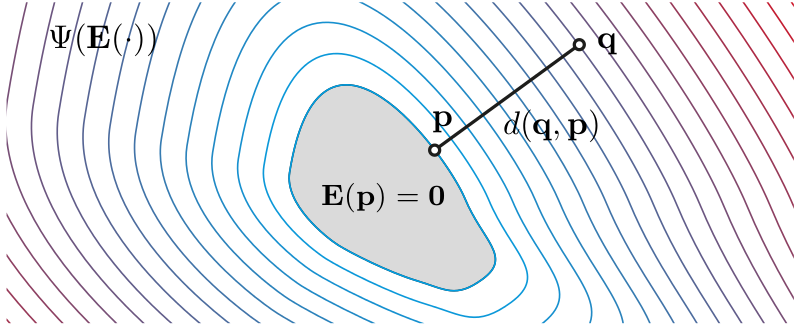
\includegraphics[scale=0.3]{pic/strain_manifold.png}
  \end{figure}
\end{frame}

\begin{frame}
  \frametitle{Nonlinear Elasticity}
  \begin{itemize}
   \item A elastic potential analogous to $\Psi(\mathbf{E}(\mathbf{q}))$
    \begin{equation*}
      \widetilde{W}(\mathbf{q})=\min_{\mathbf{p}}W(\mathbf{q}, \mathbf{p})
    \end{equation*}
    \item Quadratic distance Measures.
      \begin{equation*}
	W(\mathbf{q}, \mathbf{p})=\frac{w}{2}\|\mathbf{Aq}-\mathbf{Bp}\|^2_F+\delta_{\mathbf{C}}(\mathbf{p})
      \end{equation*}
      $\mathbf{C}$ could be any constraint $\mathbf{C}(\mathbf{q})=\mathbf{0}$ for the set of desired configurations. 
  \end{itemize}
\end{frame}

\begin{frame}
 \frametitle{Projective Implicit Euler Solver}
 \begin{itemize}
  \item Implicit integration to optimization
    \begin{equation*}
      \frac{1}{2h^2}\|\mathbf{M}^{\frac{1}{2}}(\mathbf{q}-\mathbf{s}_n)\|^2_F+\sum_i \frac{w_i}{2}\|\mathbf{A}_i
      \mathbf{S}_i\mathbf{q}-\mathbf{B}_i\mathbf{p}_i\|^2_F+\delta_{\mathbf{C}_i}(\mathbf{p}_i)
    \end{equation*}
  \item Local solve: fix position $\mathbf{q}$ and solve for auxiliary variables $\mathbf{p}_i$ independently
    \begin{equation*}
     \min_{\mathbf{p}_i} \frac{w_i}{2}\|\mathbf{A}_i
      \mathbf{S}_i\mathbf{q}-\mathbf{B}_i\mathbf{p}_i\|^2_F+\delta_{\mathbf{C}_i}(\mathbf{p}_i)
    \end{equation*}
  \item Global solve: fix auxiliary variables and solve for unknown $\mathbf{q}$
    \begin{equation*}
     (\frac{\mathbf{M}}{h^2}+\sum_i w_i\mathbf{S}_i^T\mathbf{A}_i^T\mathbf{A}_i\mathbf{S}_i)\mathbf{q}=\frac{\mathbf{M}}{h^2}
     \mathbf{s}_n + \sum_i w_i\mathbf{S}_i^T\mathbf{A}_i^T\mathbf{B}_i\mathbf{p}_i
    \end{equation*}
 \end{itemize}
\end{frame}

\begin{frame}
 \frametitle{Projective Implicit Euler Solver}
 \begin{itemize}
  \item The choice of $\mathbf{A}$ and $\mathbf{B}$
    \begin{itemize}
     \item[*] $\mathbf{A}_i=\mathbf{B}_i=\mathbf{I}$, simple but poor convergence rate.
     \item[*] $\mathbf{A}_i=\mathbf{B}_i$ as differential coordinate matrices whose null space consists of global translation.
    \end{itemize}
  \begin{figure}[h]
    \centering
    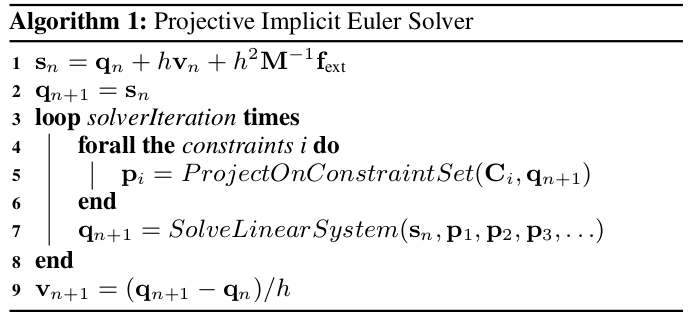
\includegraphics[scale=0.4]{pic/algorithm.png}
  \end{figure}
 \end{itemize}
\end{frame}

\begin{frame}
 \frametitle{Position Dynamics View}
 \begin{itemize}
  \item PBD actually implements a Gauss-Seidel type minimization on energy
    \begin{equation*}
     \frac{1}{2} \sum_i \|\mathbf{M}^{\frac{1}{2}}(\mathbf{S}_i\mathbf{q}-\mathbf{p}_i)\|^2_F+ \delta_{C_i}(\mathbf{p}_i)
    \end{equation*}
  \item Jacobi solver.
    \begin{itemize}
     \item[*] incompatible constraints.
     \item[*] efficient parallelization.
    \end{itemize}
 \end{itemize}
\end{frame}

\begin{frame}
 \frametitle{Continuum-Based Constraints}
 \textbf{Strain}. For 2-manifold surface
    \begin{itemize}
     \item Continuous energy
      \begin{equation*}
	E(\mathbf{f}, \mathbf{T})=\frac{w}{2}\int_S\|\nabla_S \mathbf{f}-\mathbf{T}\nabla_S \mathbf{g}\|^2_F
	+\delta_M(\mathbf{T})dA
      \end{equation*}
     \item Discrete potential
      \begin{equation*}
	W(\mathbf{q}, \mathbf{T})=\frac{w}{2}A\|\mathbf{X_fX_g}^{-1}-\mathbf{T}\|^2_F+\delta_M(\mathbf{T})
      \end{equation*}
    \end{itemize}
\end{frame}

\begin{frame}
 \frametitle{Continuum-Based Constraints}
 \textbf{Bending}.
  \begin{itemize}
   \item Continuous energy.
   \begin{equation*}
    E(\mathbf{f}, \mathbf{R})=\frac{w}{2}\int_S\|\Delta_S\mathbf{f}-\mathbf{R}\Delta_S\mathbf{g}\|^2_2
    +\delta_{SO(3)}(\mathbf{R})dA
   \end{equation*}
   \item Discrete potential
   \begin{equation*}
    W(\mathbf{q}, \mathbf{R})=\frac{w}{2}A\|\mathbf{X_fc}-\mathbf{RX_gc}\|^2_2+\delta_{SO(3)}(\mathbf{R})
   \end{equation*}
  \end{itemize}
\end{frame}

\begin{frame}
 \frametitle{Conclusion}
 %\TikzDraw{
    %\visible<1> {\node at (2,-2) {\parbox[t]{\textwidth}{
     %   \Large$\pi(x_1) = \pi(x_2) = x$}
     % }; 
    %}
   % \visible<1> {\node at (7, -3) {\parbox[t]{\textwidth}{
    %      $\alpha\circ \tau = -\alpha\\ cos(\alpha)=cos(-\alpha)$
    %    }};
   % }
 %}
\end{frame}

\begin{frame}
  \frametitle{Conclusion}
  \begin{itemize}
   \item handling non-linearity.
   \item discontinuous galerkin.
   \item mesh dependent.
  \end{itemize}
\end{frame}

\end{document}
